\section{Modélisation du système (UML)}
\label{chap:modelisation}

Cette section traduit en modèles UML le cahier des charges formalisé à la section~\ref{chap:besoins}. Il présente successivement la vue statique des acteurs et des fonctionnalités (cas d'utilisation), le modèle de données conceptuel (classes du domaine), les comportements dynamiques des scénarios les plus structurants (séquences) et le circuit de validation hiérarchique (activité). Chaque élément de modélisation est explicitement tracé vers les identifiants d'exigences (\texttt{EF-*}) introduits à la section~\ref{chap:besoins}.

\subsection{Vue des cas d'utilisation}
\label{sec:cas_utilisation}
Les Figures~\ref{fig:cas_utilisation_1} et~\ref{fig:cas_utilisation_2} présentent le diagramme de cas d'utilisation global, scindé en deux vues pour la lisibilité. Les acteurs retenus sont les trois rôles RBAC de \texttt{ENF-SEC-03} (\texttt{DAKAR\_AGENT}, \texttt{BAMAKO\_CHEF}, \texttt{ADMIN}), plus le Planificateur ETL, un acteur non humain porté par Apache Airflow. Les vingt-quatre cas d'utilisation couvrent les exigences fonctionnelles \textit{Must} et \textit{Should} des six modules M1 à M6 ; chaque bulle porte son identifiant \texttt{EF-*} pour rester traçable vers la section~\ref{chap:besoins}. Le Planificateur ETL apparaît comme un acteur à part entière, même non humain, parce qu'il déclenche le pipeline d'ingestion (\texttt{EF-ETL-01}) de façon autonome, sur le temps plutôt que sur une action utilisateur. Les relations «\,include\,» couvrent les sous-fonctions systématiquement mobilisées (contrôles de doublon et de ration à chaque saisie) ; la relation «\,extend\,», réservée à la classification de flotte (\texttt{EF-DSH-03}), exprime un comportement optionnel. Le solde de caisse n'est pas l'objet d'un cas de saisie : c'est une valeur dérivée (total des entrées moins total des sorties), recalculée à chaque transaction saisie (\texttt{EF-SDR-01}). L'Agent Dakar saisit donc des transactions, dépenses ou entrées, et consulte le solde qui en résulte sur le tableau de bord (\texttt{EF-DSH-01}) ; une note relie les deux cas sur chaque vue.

\begin{figure}[H]
    \centering
    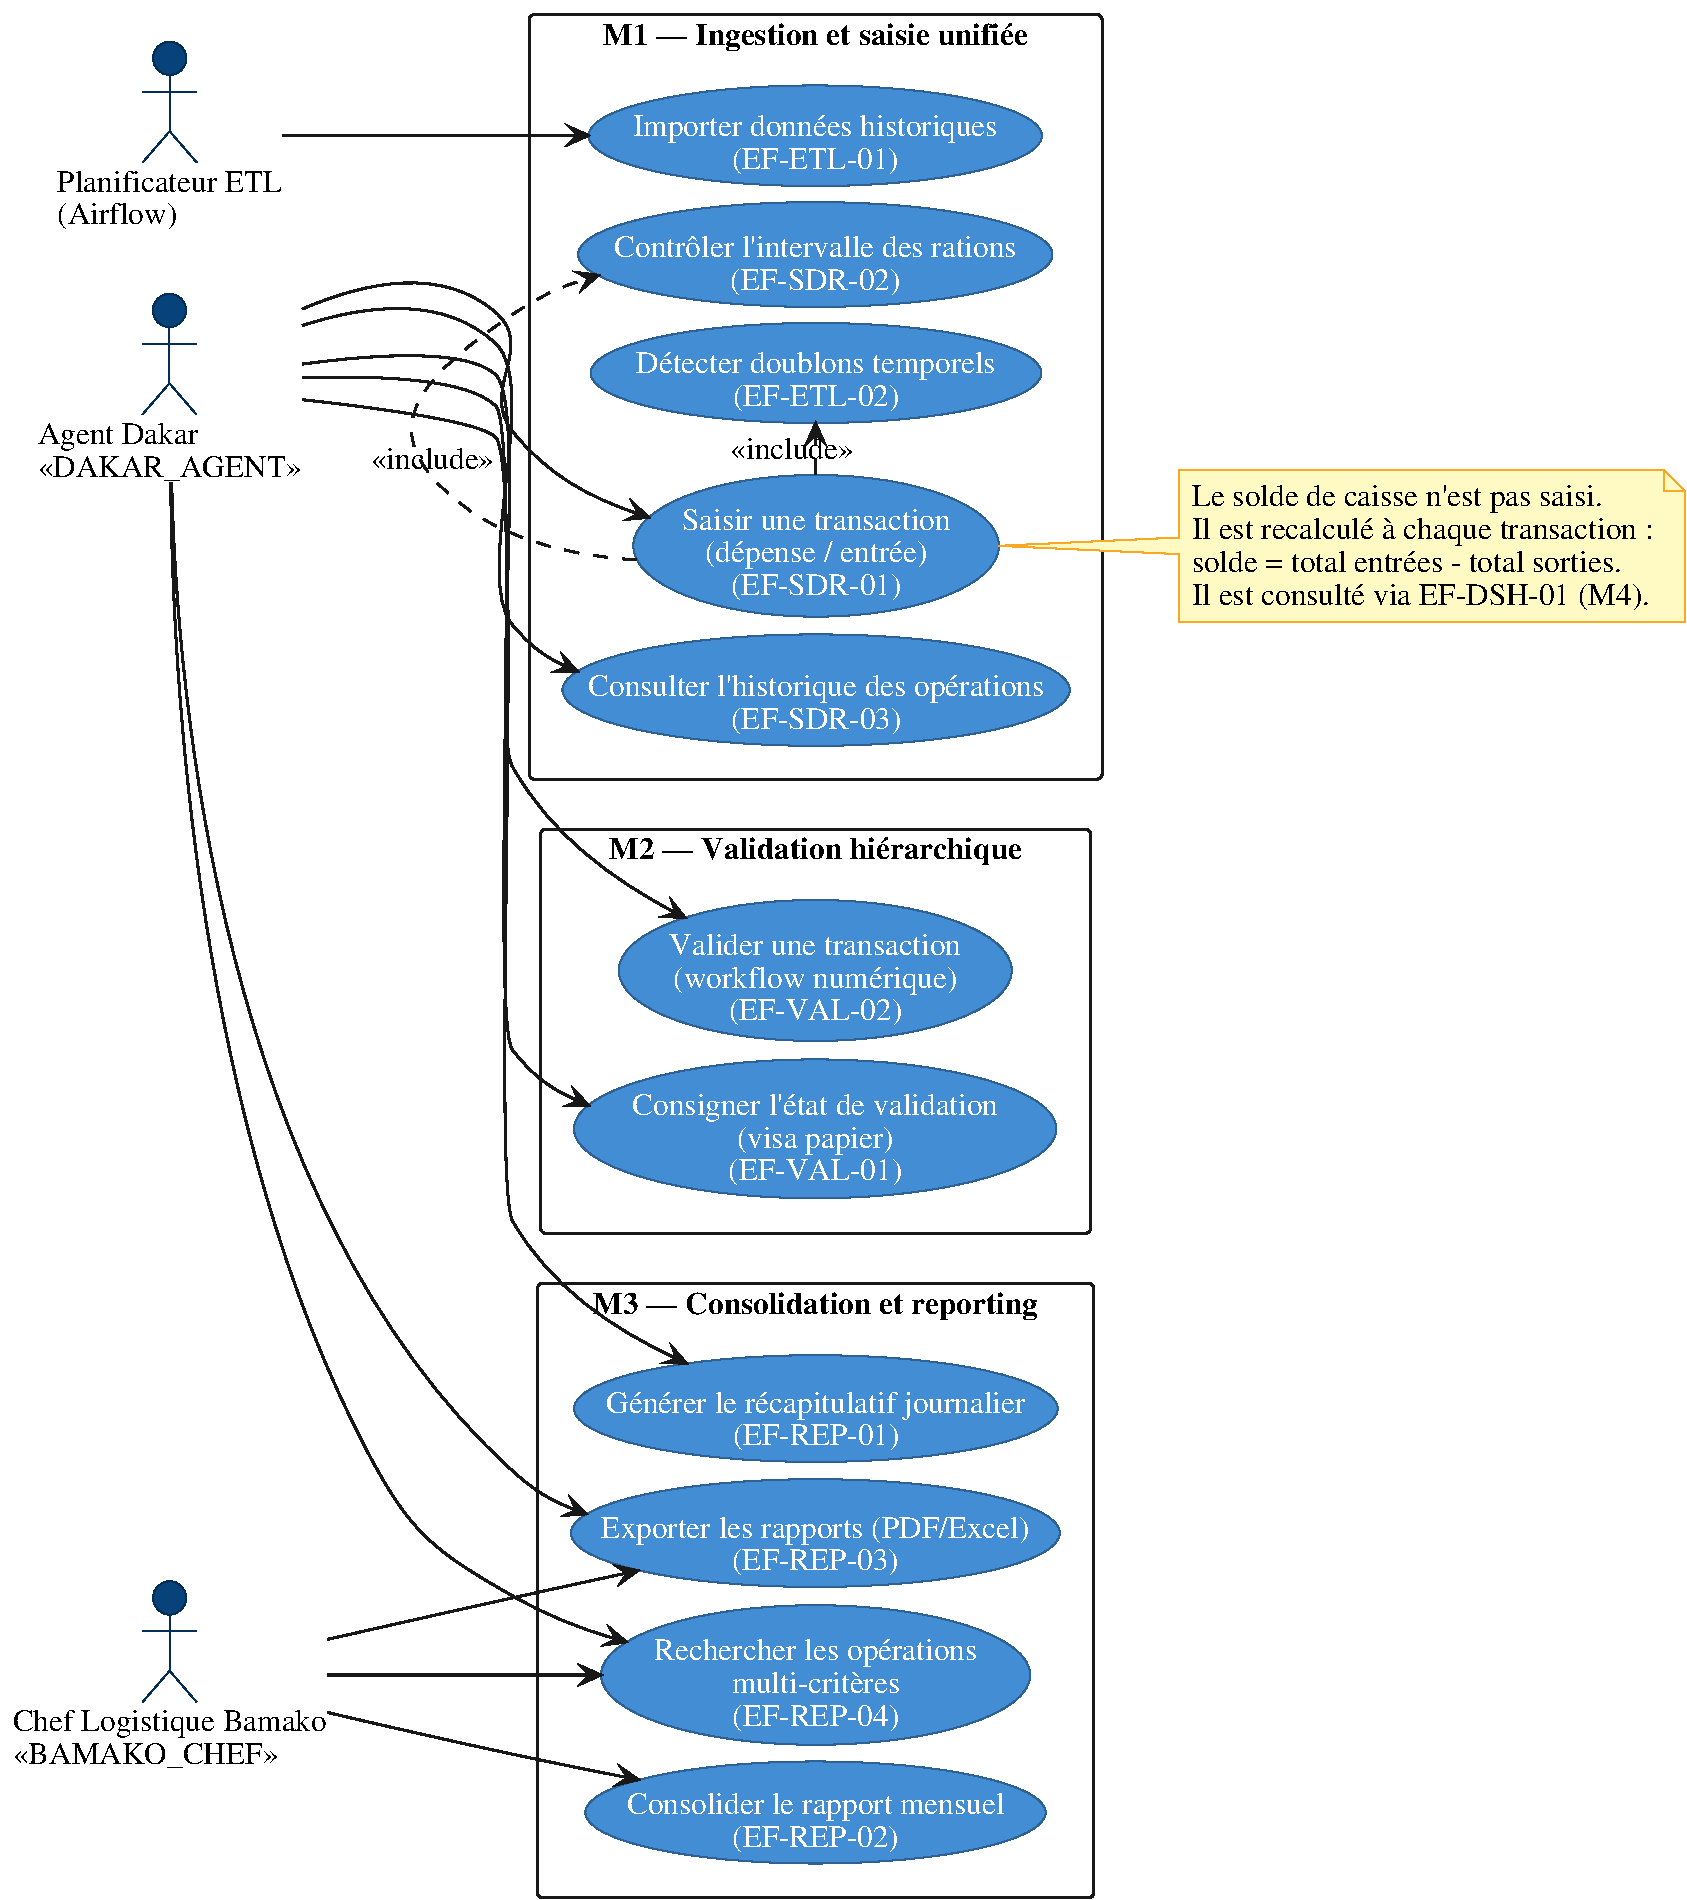
\includegraphics[width=\textwidth,height=0.88\textheight,keepaspectratio]{figures/fig_cas_utilisation_m1_m3.pdf}
    \caption{Diagramme de cas d'utilisation, modules M1 à M3 (Ingestion, Validation, Reporting), plateforme SOYAFF}
    \label{fig:cas_utilisation_1}
    \source{Schéma de l'auteur}
\end{figure}

\begin{figure}[H]
    \centering
    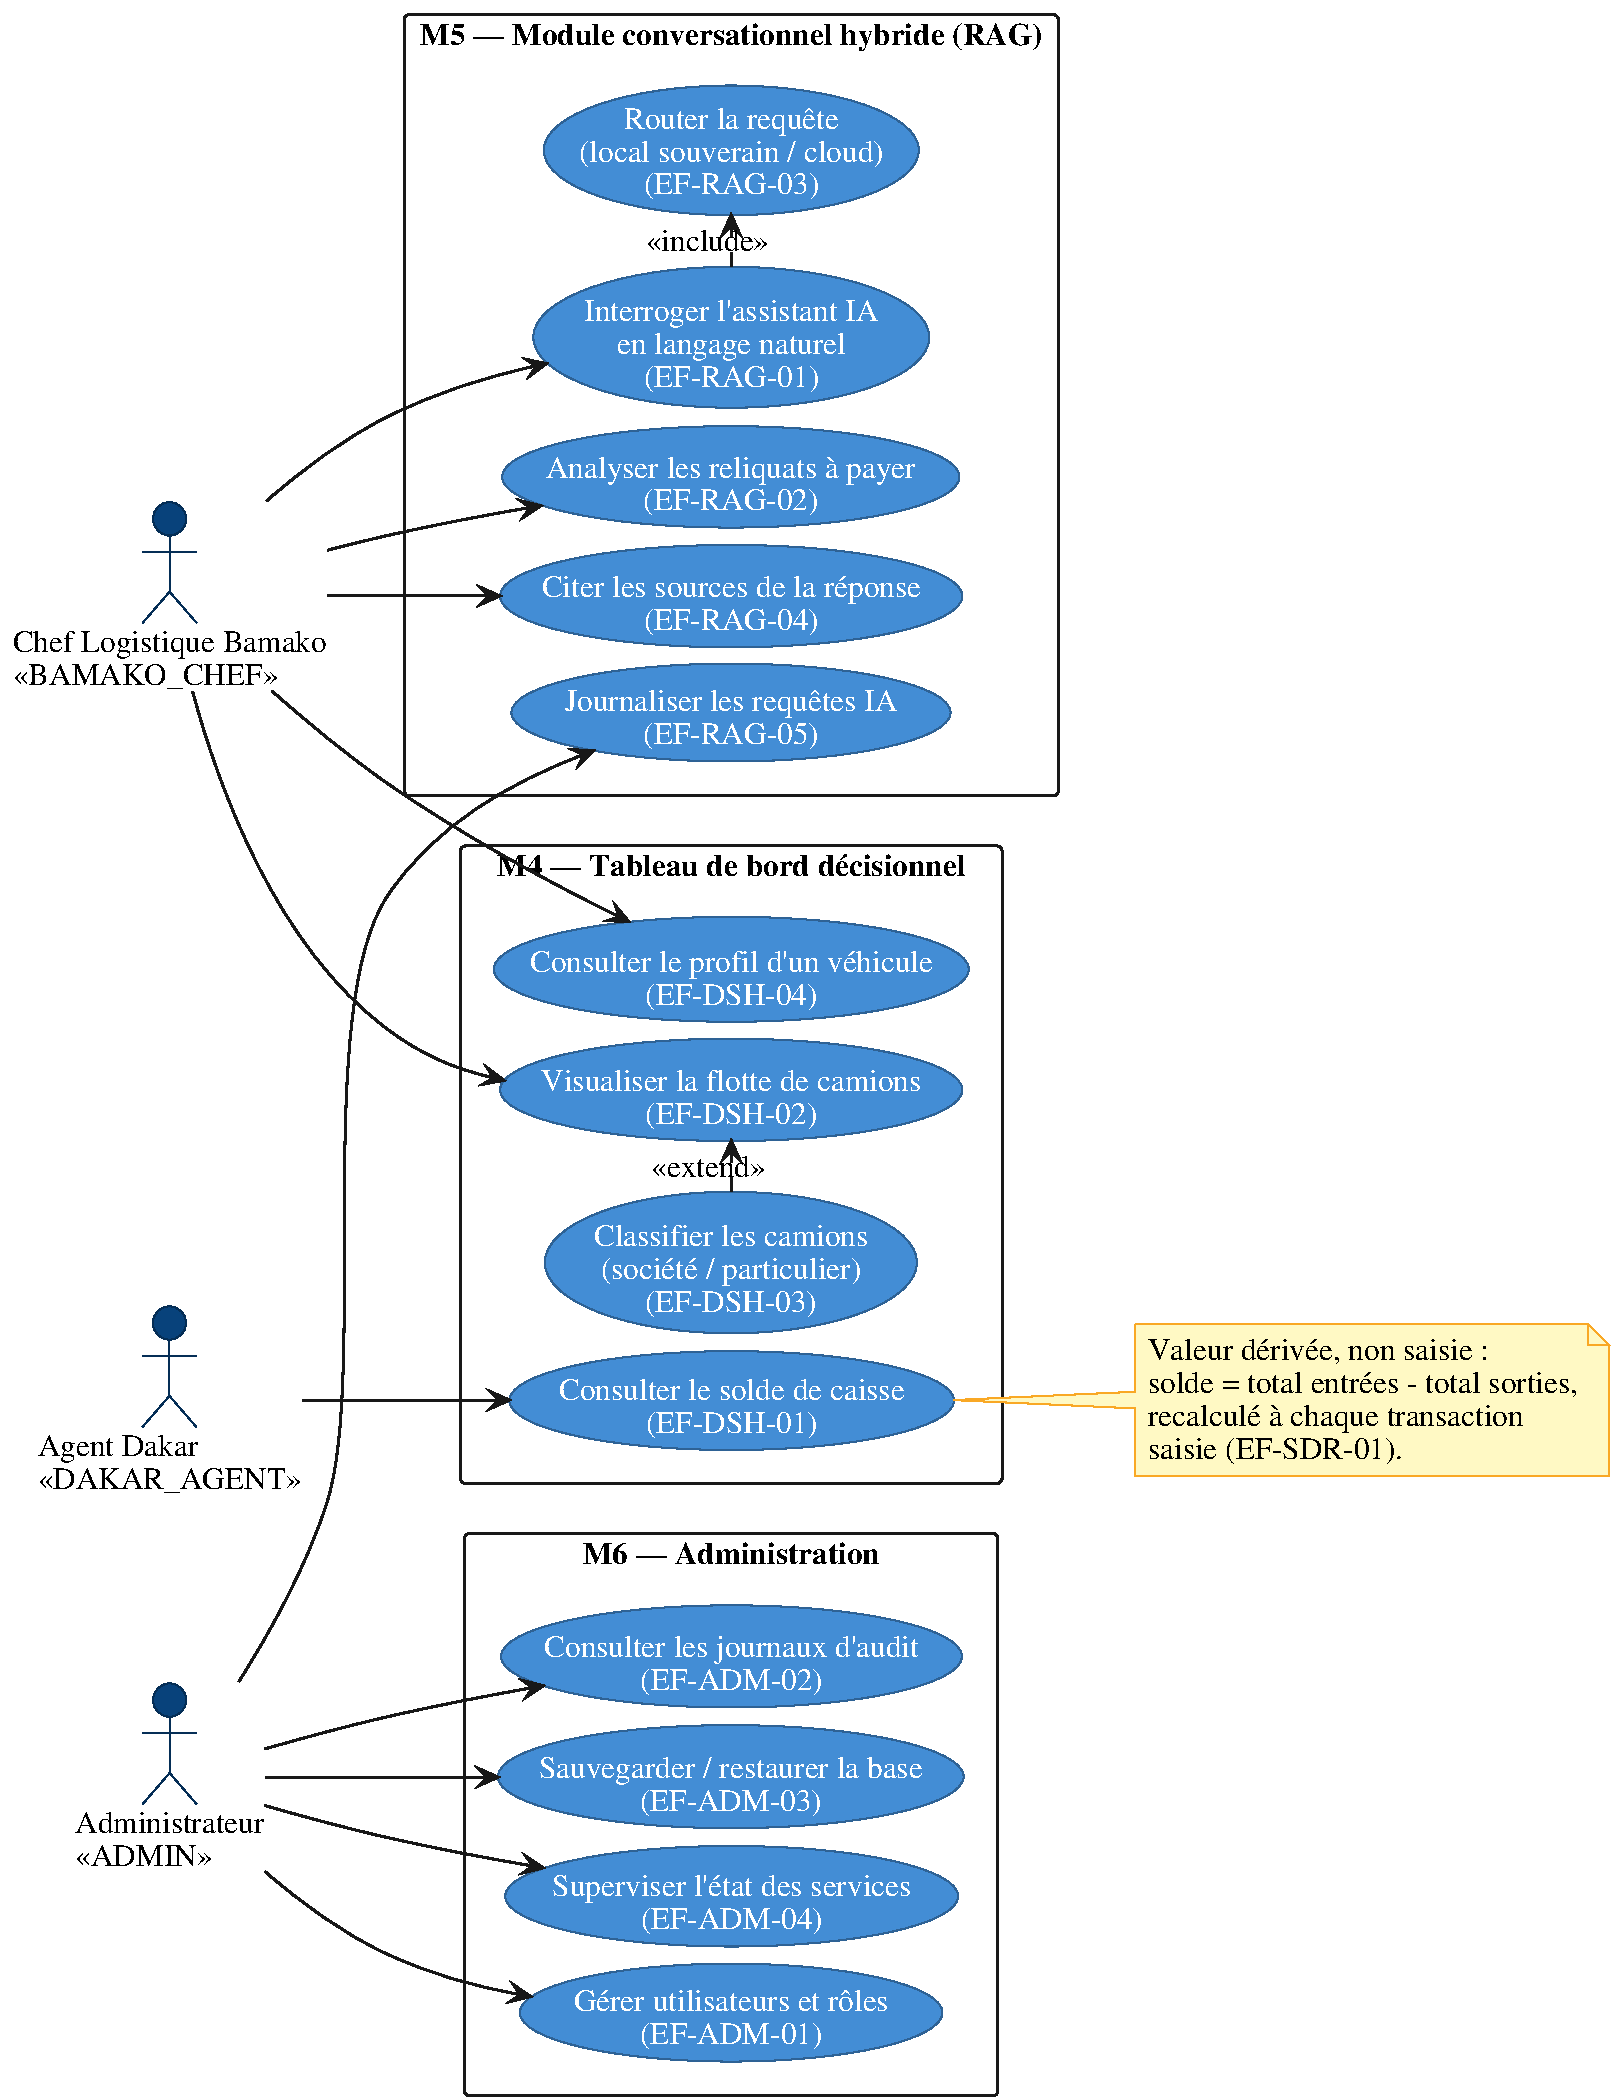
\includegraphics[width=\textwidth,height=0.88\textheight,keepaspectratio]{figures/fig_cas_utilisation_m4_m6.pdf}
    \caption{Diagramme de cas d'utilisation, modules M4 à M6 (Tableau de bord, RAG, Administration), plateforme SOYAFF}
    \label{fig:cas_utilisation_2}
    \source{Schéma de l'auteur}
\end{figure}

\subsection{Modèle de classes du domaine}
\label{sec:classes_domaine}
Le diagramme de classes du domaine métier (Figure~\ref{fig:classes_domaine}) modélise les concepts manipulés par la plateforme, à un niveau d'abstraction conceptuel et non celui du schéma physique de base de données présenté à la section~\ref{chap:architecture}. Les noms de classes et d'attributs sont volontairement alignés sur les tables et colonnes réelles de la base PostgreSQL, afin d'assurer la cohérence entre l'analyse et la réalisation. La classe \texttt{Validation} y figure avec le stéréotype \guillemotleft~conceptuel~\guillemotright~: elle matérialise les exigences \texttt{EF-VAL-01/02} sans préjuger d'une persistance déjà implémentée, cet aspect étant traité au chapitre~\ref{chap:realisation}.

Le modèle s'articule autour de la classe centrale \texttt{Transaction}, qui matérialise tout mouvement financier ou opérationnel. Une \texttt{Transaction} \emph{concerne} un \texttt{Camion} (multiplicité 1 côté camion, chaque camion pouvant porter un nombre indéterminé de transactions), lui-même \emph{conduit} par un \texttt{Chauffeur} : cette chaîne permet de reconstituer le coût réel par véhicule et par chauffeur, indicateur central absent du système actuel (cf. §\ref{sec:recueil}). La classe \texttt{BonLivraison} agrège les transactions relatives à un même chargement et est reliée aux \texttt{Produit} transportés par une association plusieurs-à-plusieurs, un bon regroupant plusieurs références et une référence figurant sur plusieurs bons. Cette association porte une donnée qui n'appartient ni au bon ni au produit, la quantité livrée : elle est donc modélisée par la classe d'association \texttt{BonLivraisonProduit}, rattachée au lien entre les deux classes. L'attribut \texttt{/solde\_progressif} de \texttt{Transaction} est noté comme attribut dérivé : il n'est jamais saisi, mais calculé à partir des entrées et des sorties. Enfin, la classe \texttt{Validation}, ici purement conceptuelle, s'attache à la \texttt{Transaction} qu'elle qualifie sans en présumer la persistance physique. Les classes \texttt{Utilisateur}, \texttt{RequeteIA} et \texttt{AuditLog} constituent le socle transverse de sécurité et de traçabilité (RBAC, journalisation IA et piste d'audit) exigé par les \texttt{ENF-SEC} et \texttt{EF-RAG-05}. L'ensemble \texttt{CategorieOperation} est modélisé comme une énumération (et non une entité), reflétant son statut de colonne typée dans le schéma relationnel.

\begin{landscape}
\begin{figure}[p]
    \centering
    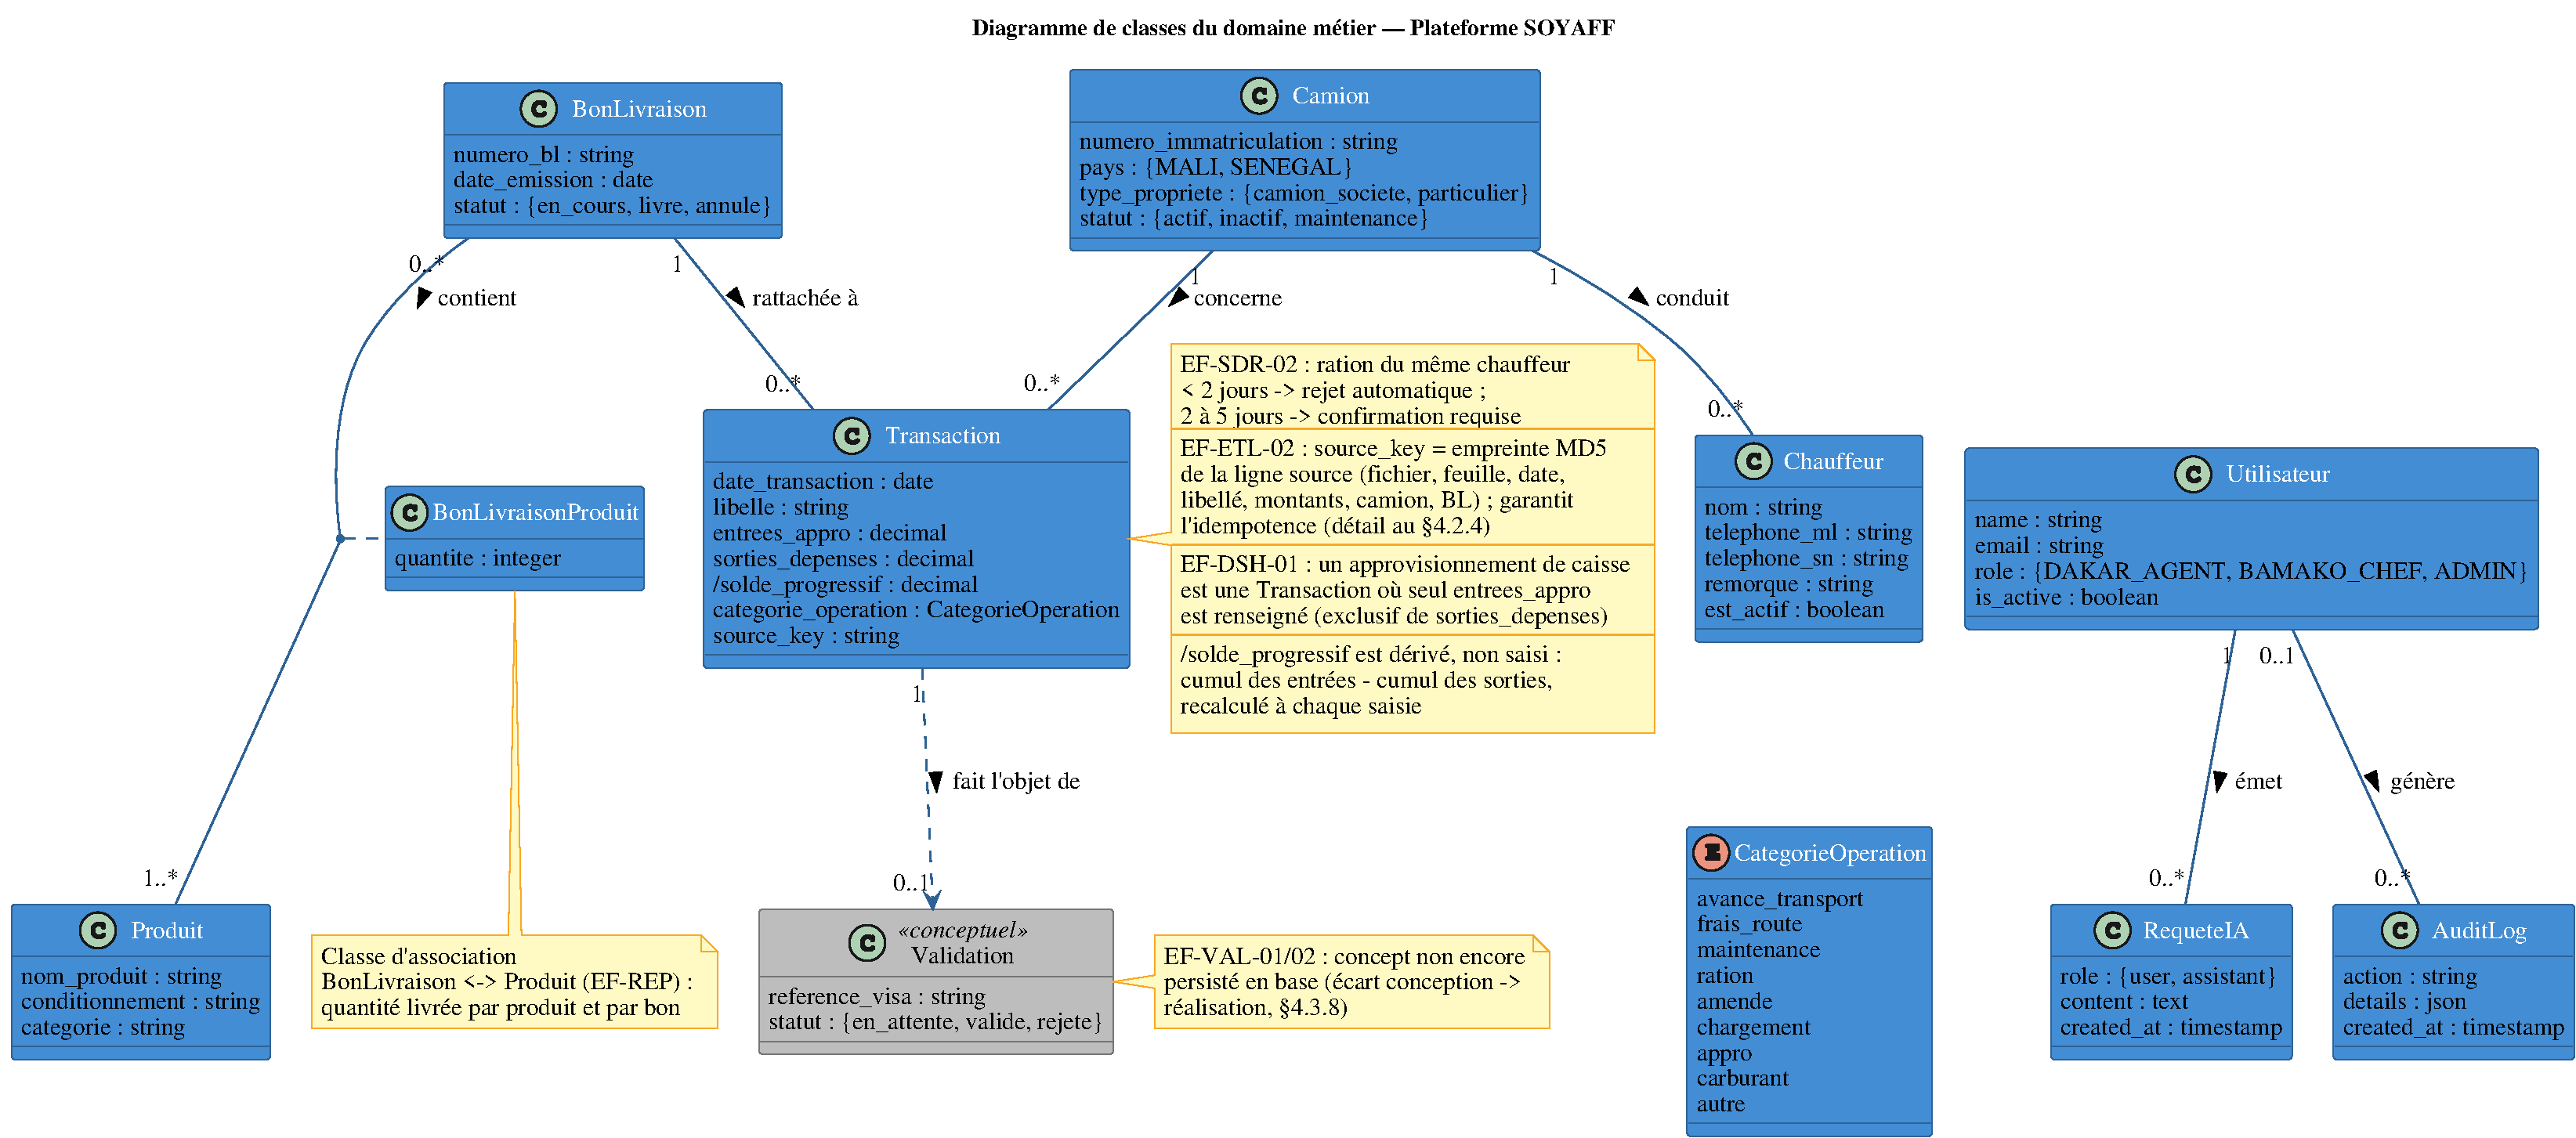
\includegraphics[width=\linewidth,height=0.86\textheight,keepaspectratio]{figures/fig_classes_domaine.pdf}
    \caption{Diagramme de classes du domaine métier, plateforme SOYAFF}
    \label{fig:classes_domaine}
    \source{Schéma de l'auteur}
\end{figure}
\end{landscape}

\subsection{Comportements dynamiques}
\label{sec:sequences}
Les deux scénarios suivants ont été retenus pour leur caractère structurant : le premier opérationnalise les garde-fous métier de la saisie (§\ref{sec:recueil}), le second matérialise la définition d'architecture \guillemotleft~hybride~\guillemotright~qui porte l'hypothèse H2.

\subsubsection{Séquence de saisie d'une dépense avec contrôles}
\label{subsec:seq_saisie}
La Figure~\ref{fig:seq_saisie} détaille le scénario de saisie d'une dépense, avec ses deux garde-fous : la détection de doublons temporels (\texttt{EF-ETL-02}) et le contrôle de l'intervalle entre deux rations (\texttt{EF-SDR-02}), modélisés par des fragments combinés \texttt{alt}.

\begin{figure}[H]
    \centering
    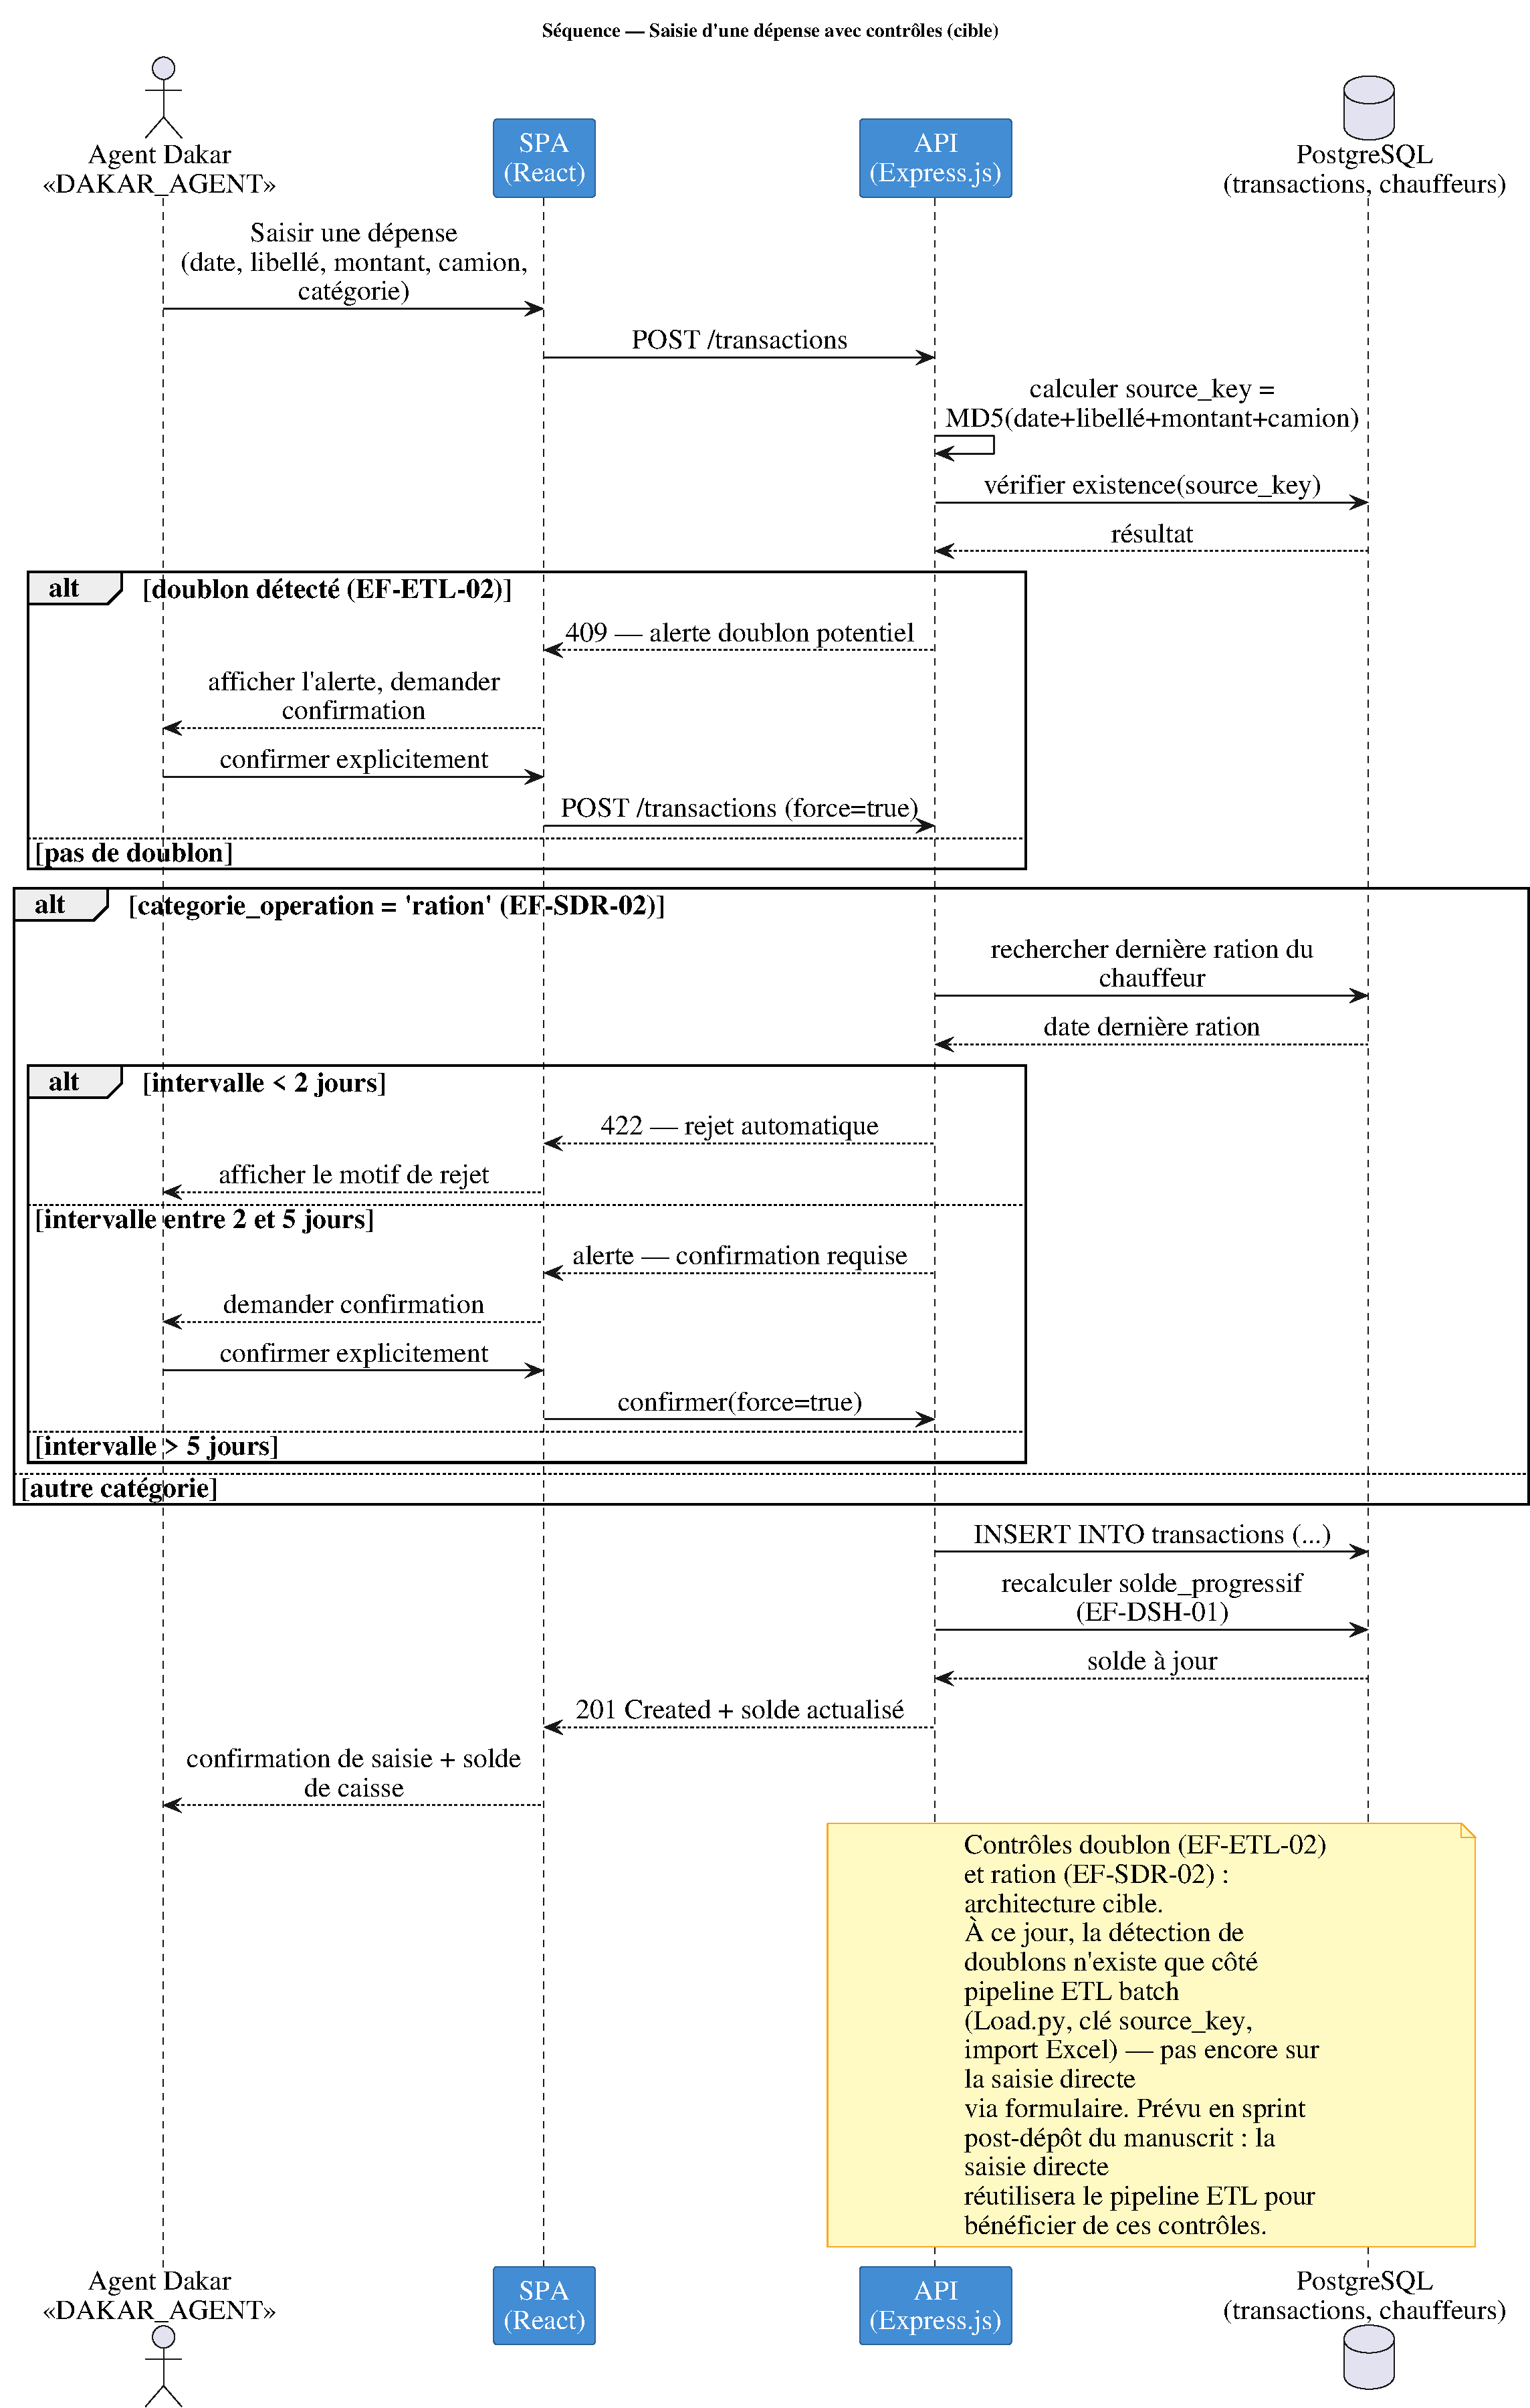
\includegraphics[width=\textwidth,height=0.88\textheight,keepaspectratio]{figures/fig_seq_saisie_controles.pdf}
    \caption{Séquence : saisie d'une dépense avec contrôles}
    \label{fig:seq_saisie}
    \source{Schéma de l'auteur}
\end{figure}

\subsubsection{Séquence de requête RAG avec routage hybride}
\label{subsec:seq_rag}
La Figure~\ref{fig:seq_rag} illustre le traitement d'une requête en langage naturel adressée à l'agent conversationnel, depuis sa soumission jusqu'à la restitution de la réponse. Le routage entre chemin local souverain et chemin cloud (\texttt{EF-RAG-03}) y est représenté par un fragment \texttt{alt} conditionné par l'analyse de sensibilité réalisée par l'orchestrateur n8n.

\begin{landscape}
\begin{figure}[p]
    \centering
    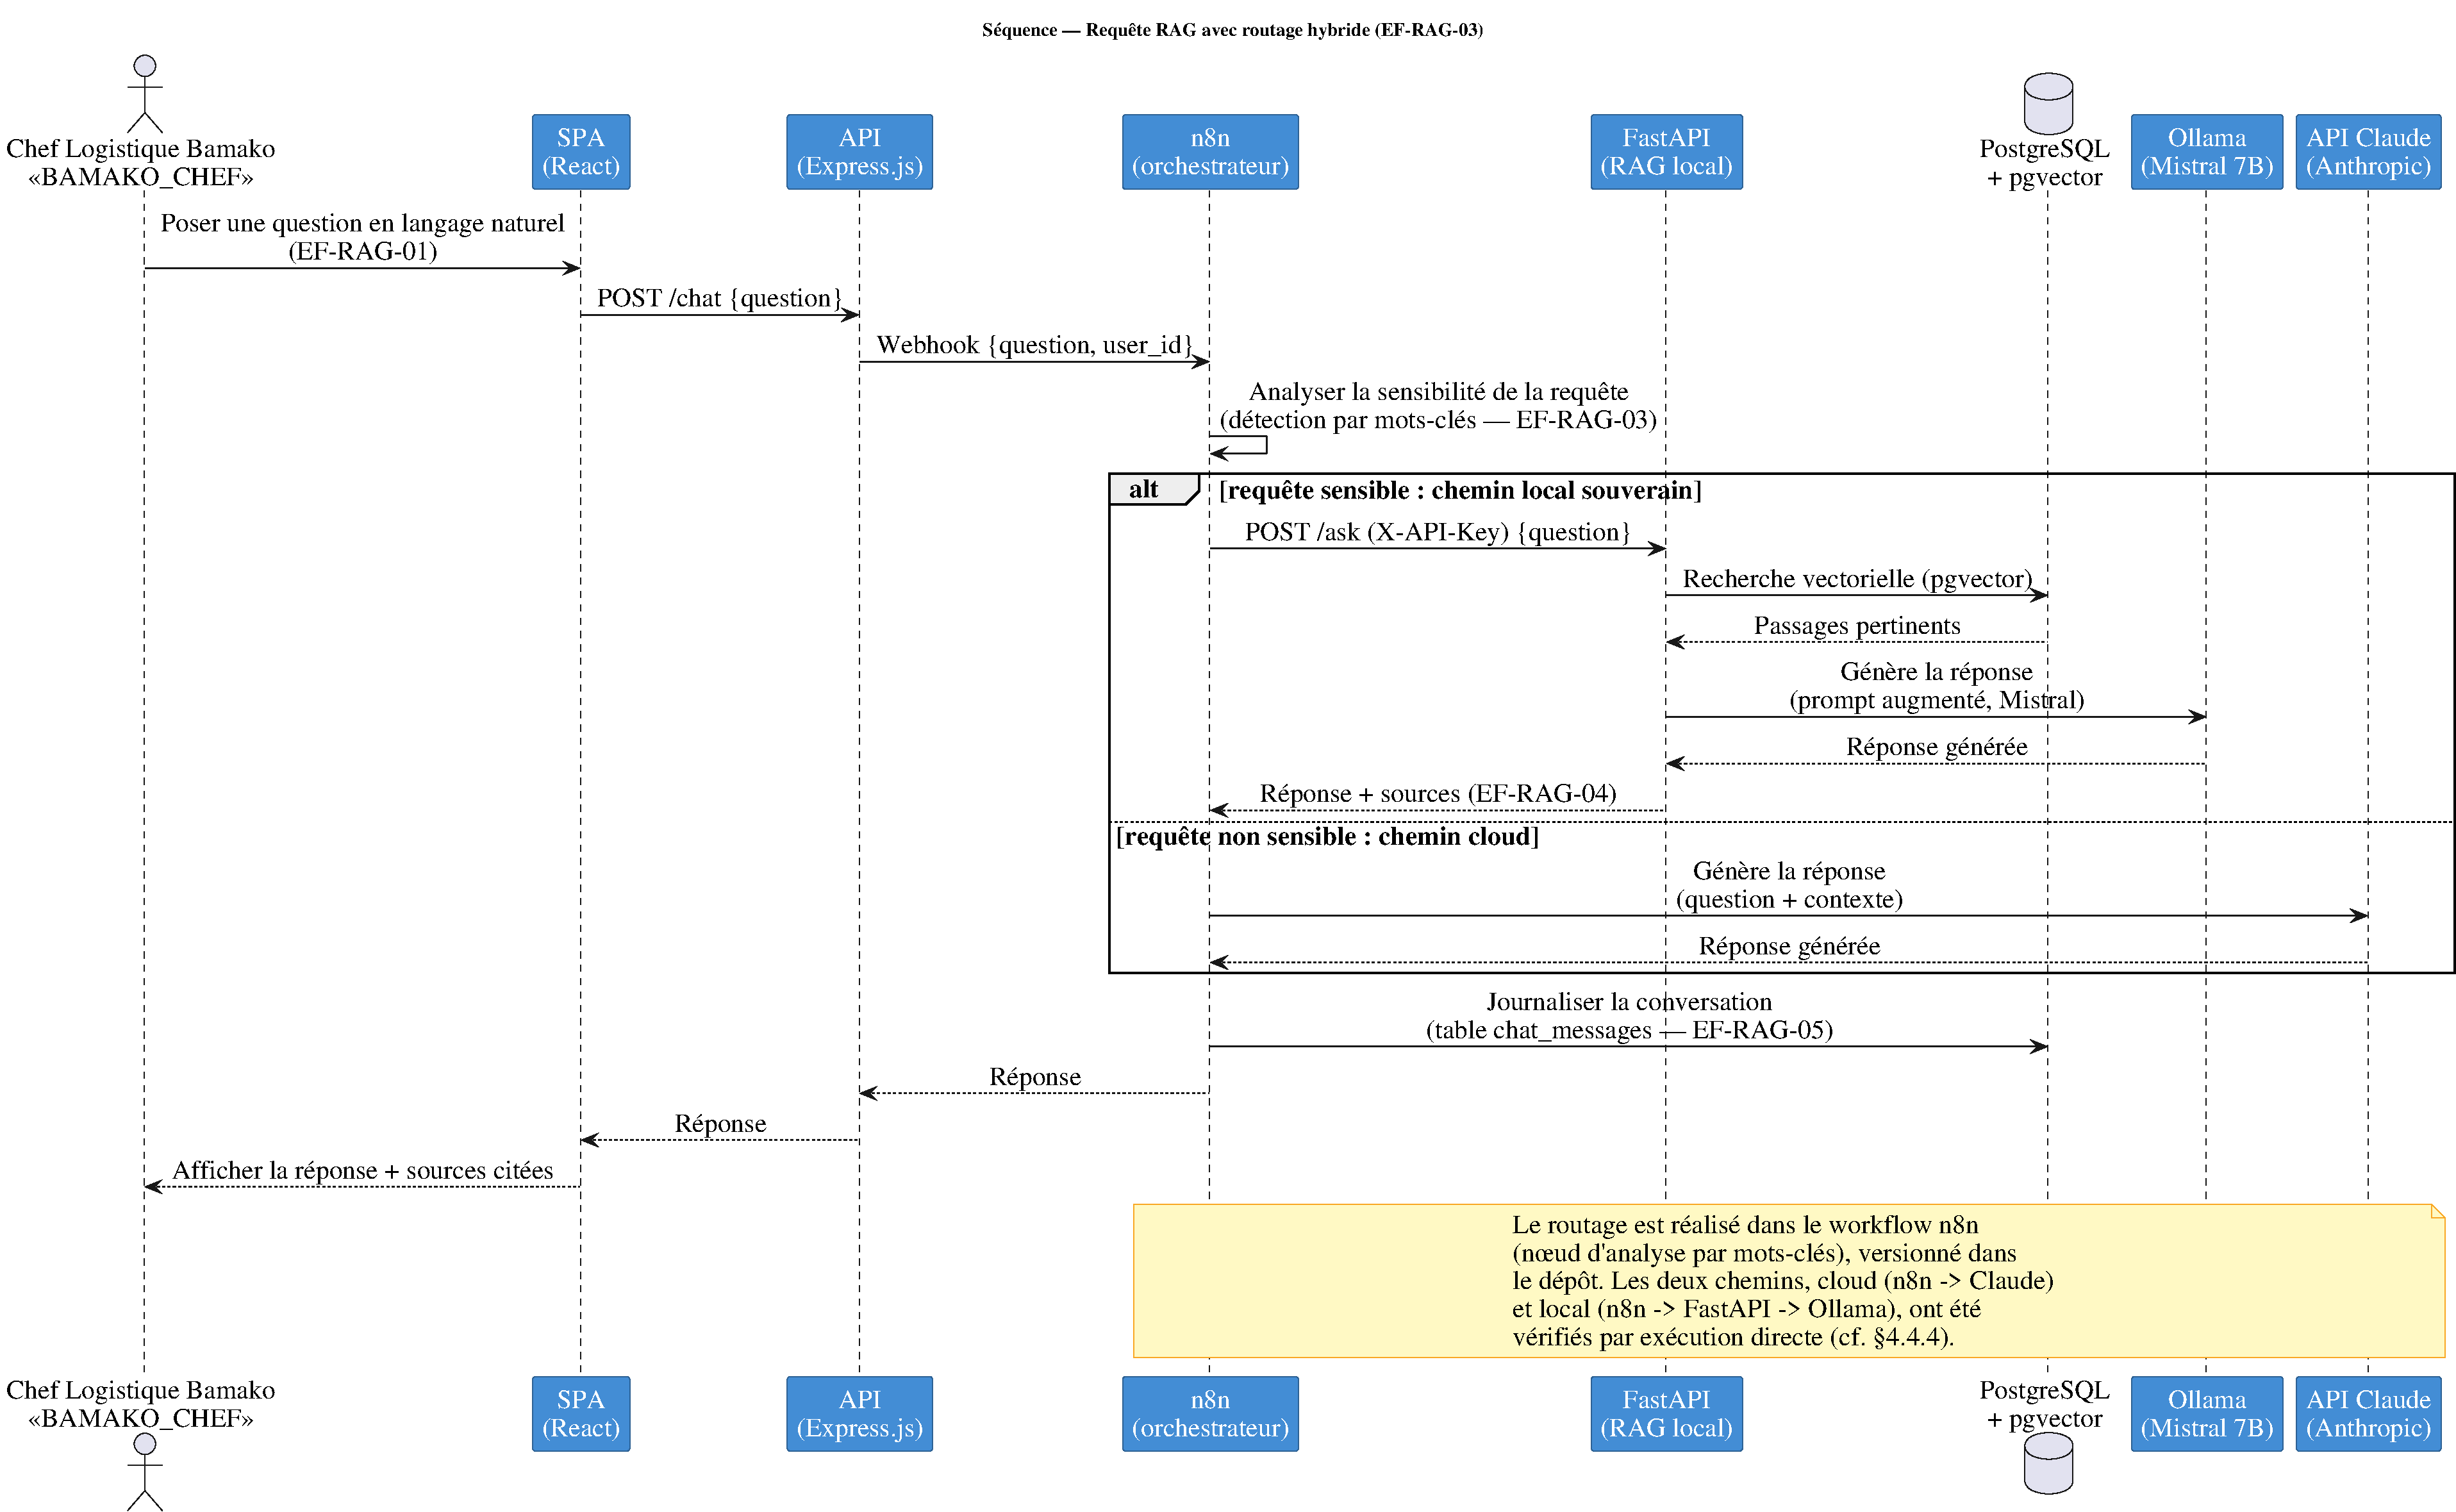
\includegraphics[width=\linewidth,height=0.86\textheight,keepaspectratio]{figures/fig_seq_rag_hybride.pdf}
    \caption{Séquence : requête RAG avec routage hybride}
    \label{fig:seq_rag}
    \source{Schéma de l'auteur}
\end{figure}
\end{landscape}

\subsection{Workflow de validation}
\label{sec:activite_validation}
Les deux séquences précédentes décrivent des interactions synchrones, centrées sur une requête unique. Le processus de validation, lui, est un flux de travail asynchrone avec plusieurs acteurs et des points de décision : le diagramme d'activité est le formalisme adapté.

Les Figures~\ref{fig:activite_validation_actuelle} et~\ref{fig:activite_validation_cible} présentent, sous forme de diagrammes d'activité à couloirs, le circuit de validation observé sur le terrain et le circuit dématérialisé cible. Le premier correspond à l'exigence \textit{Must} \texttt{EF-VAL-01} ; le second, à l'exigence \textit{Should} \texttt{EF-VAL-02}, dont la priorisation reflète le maintien du circuit papier comme référence juridiquement opposable durant la phase de transition (§\ref{sec:synthese_tracabilite}).

\begin{figure}[H]
    \centering
    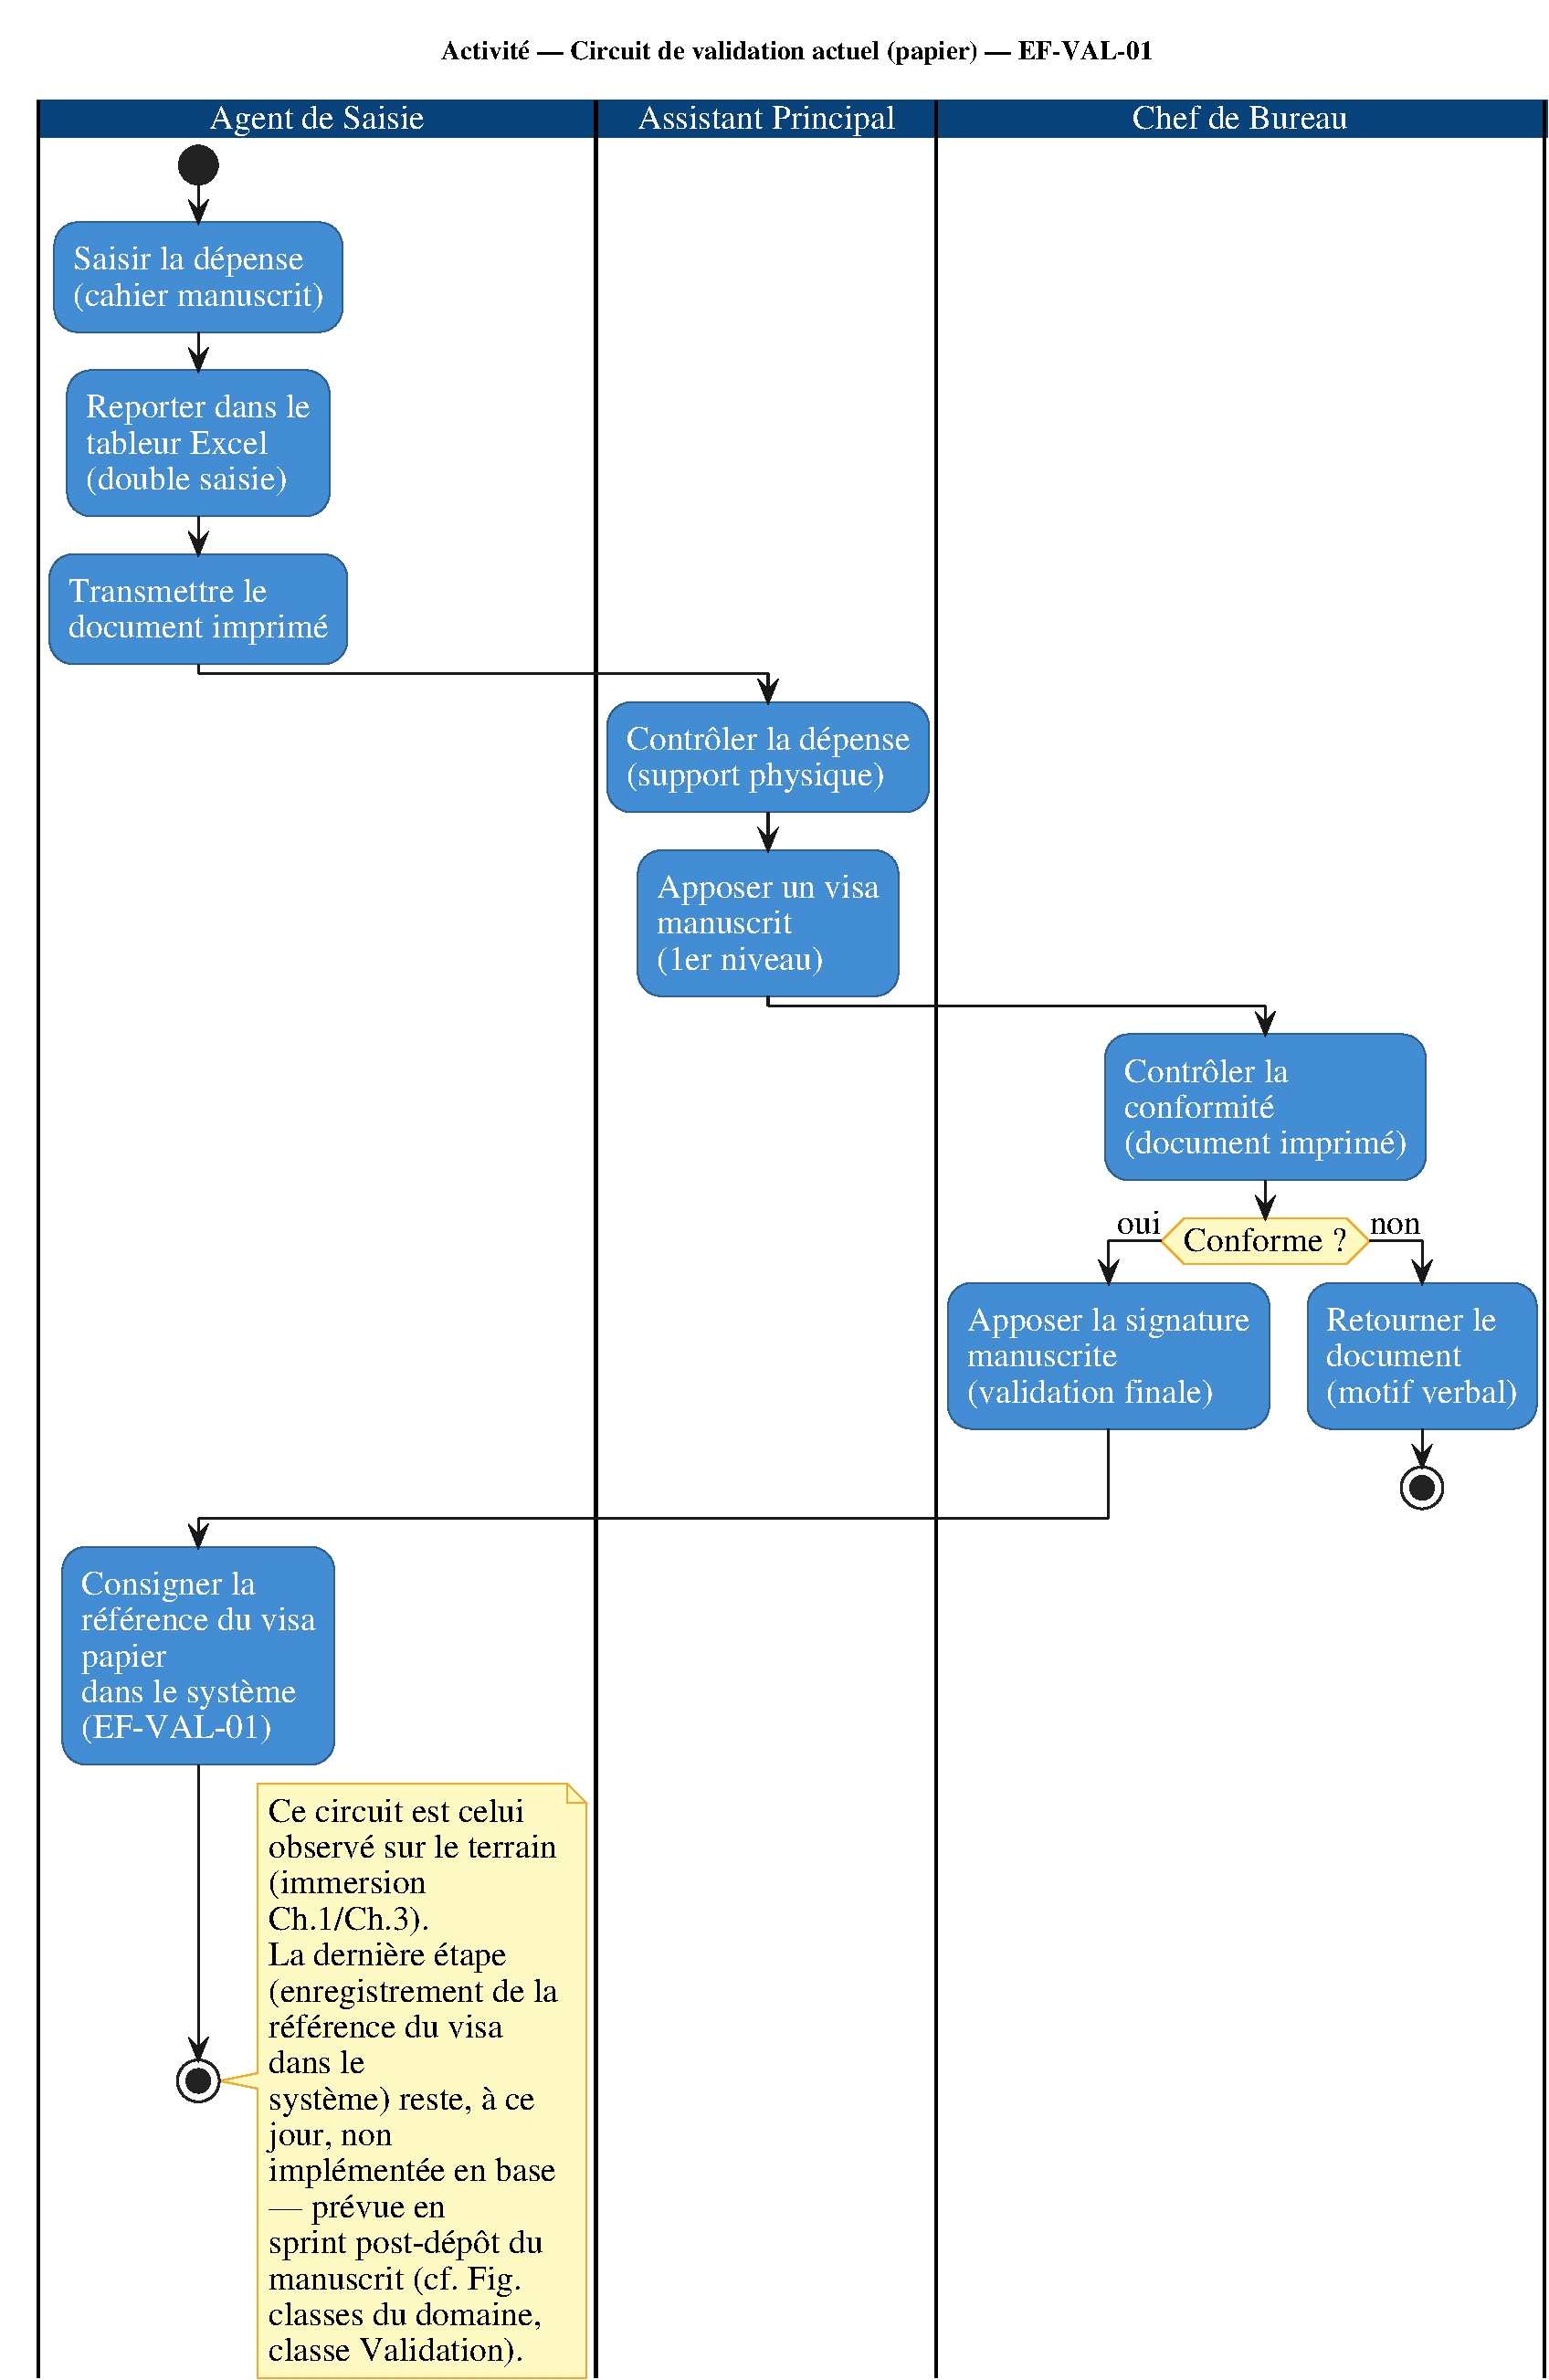
\includegraphics[width=\textwidth,height=0.88\textheight,keepaspectratio]{figures/fig_activite_validation_actuelle.pdf}
    \caption{Activité : circuit de validation actuel (papier)}
    \label{fig:activite_validation_actuelle}
    \source{Schéma de l'auteur}
\end{figure}

\begin{figure}[H]
    \centering
    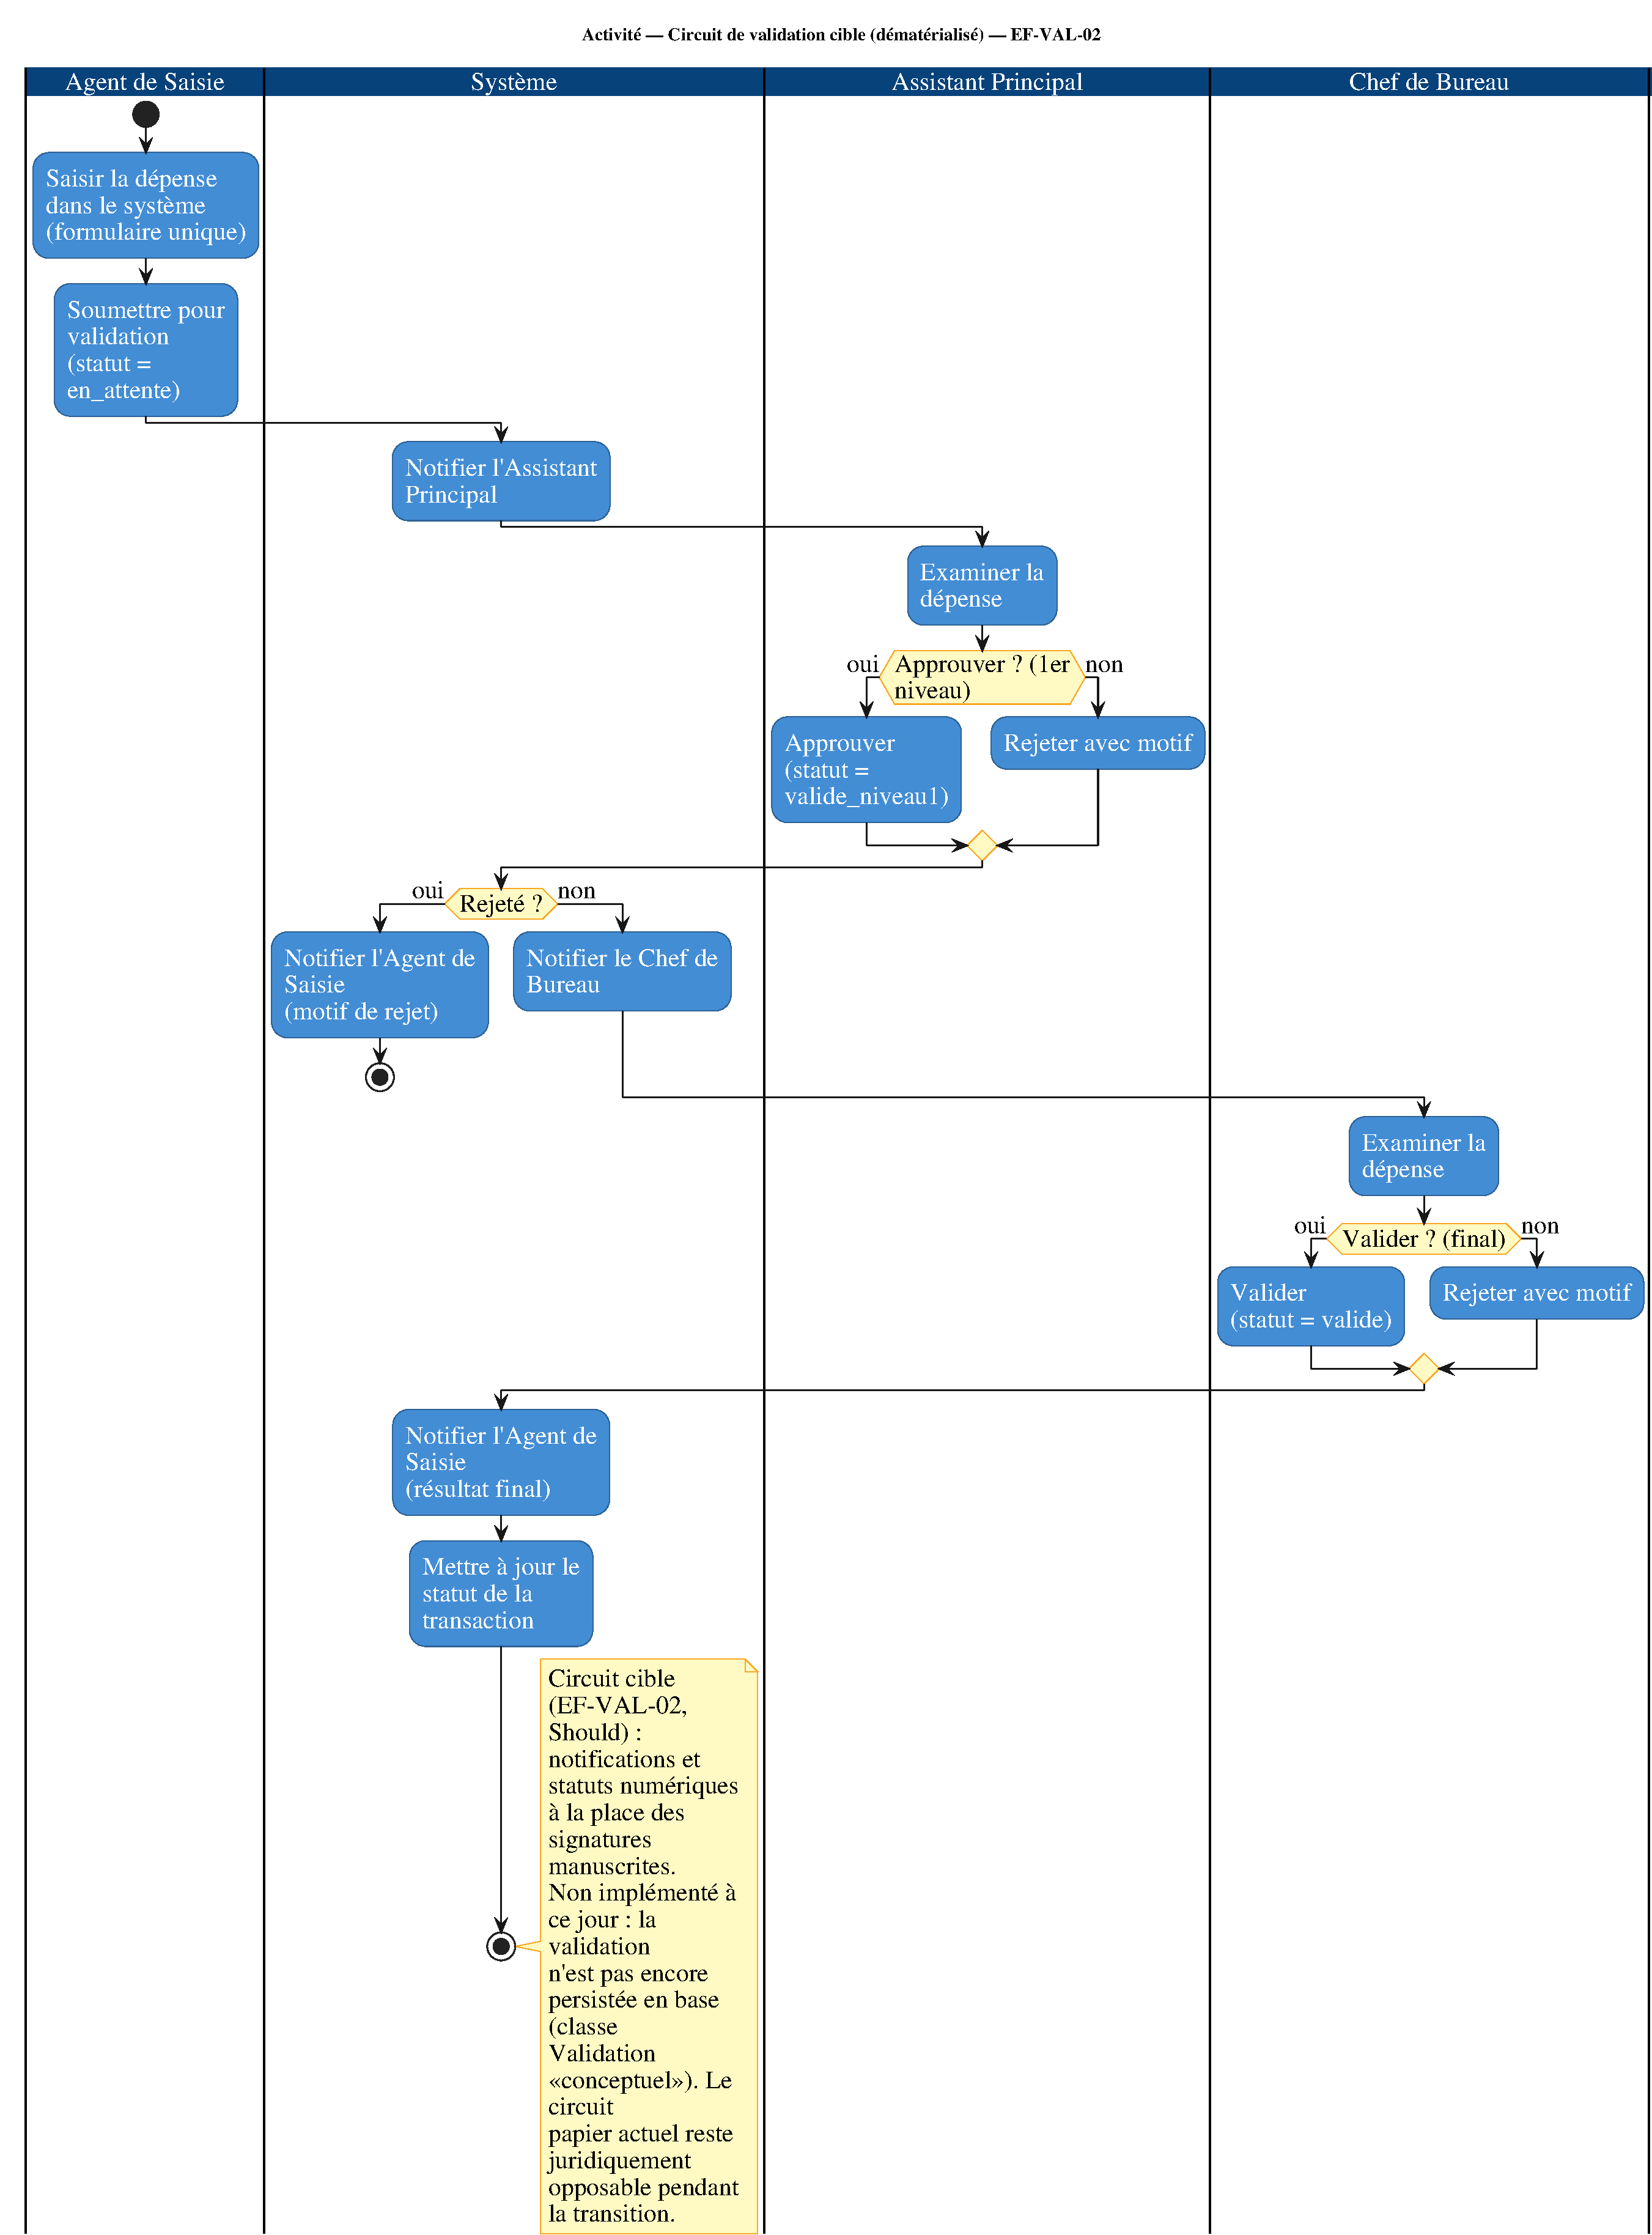
\includegraphics[width=\textwidth,height=0.88\textheight,keepaspectratio]{figures/fig_activite_validation_cible.pdf}
    \caption{Activité : circuit de validation cible (dématérialisé)}
    \label{fig:activite_validation_cible}
    \source{Schéma de l'auteur}
\end{figure}

